% Figure: Coordination Patterns detected by Agent 3b
% Data source: Sutra Pipeline database, 17,955 analyzed papers
% Usage: % Figure: Coordination Patterns detected by Agent 3b
% Data source: Sutra Pipeline database, 17,955 analyzed papers
% Usage: % Figure: Coordination Patterns detected by Agent 3b
% Data source: Sutra Pipeline database, 17,955 analyzed papers
% Usage: % Figure: Coordination Patterns detected by Agent 3b
% Data source: Sutra Pipeline database, 17,955 analyzed papers
% Usage: \input{figures/coordination-patterns.tex}

\begin{figure}[t]
\centering
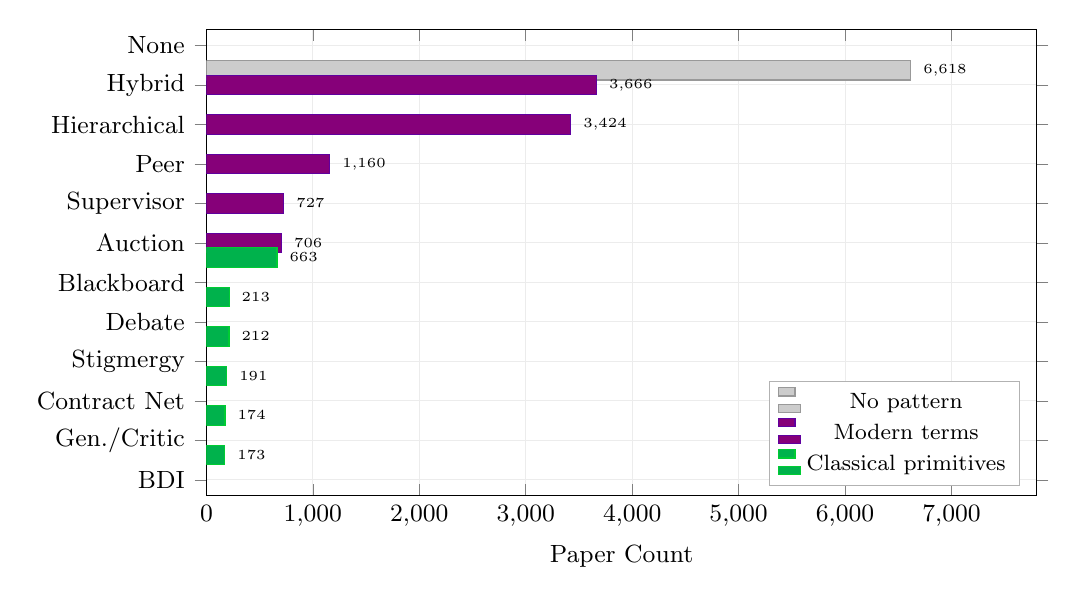
\begin{tikzpicture}
\begin{axis}[
    xbar,
    width=\columnwidth,
    height=7.5cm,
    xlabel={Paper Count},
    xlabel style={font=\small},
    xmin=0, xmax=7800,
    ytick={0,1,2,3,4,5,6,7,8,9,10,11},
    yticklabels={
        {None},
        {Hybrid},
        {Hierarchical},
        {Peer},
        {Supervisor},
        {Auction},
        {Blackboard},
        {Debate},
        {Stigmergy},
        {Contract Net},
        {Gen./Critic},
        {BDI}
    },
    yticklabel style={font=\small},
    y dir=reverse,
    bar width=7pt,
    nodes near coords,
    nodes near coords style={font=\tiny, anchor=west},
    every node near coord/.append style={xshift=1pt},
    enlarge y limits={abs=0.4},
    grid=major,
    grid style={gray!15},
    xticklabel style={font=\small},
    point meta=explicit symbolic,
    legend style={
        at={(0.98,0.02)},
        anchor=south east,
        font=\footnotesize,
        draw=black!30,
    },
]

% None (gray)
\addplot[fill=black!20, draw=black!40] coordinates {
    (6618,0) [6{,}618]
};
\addlegendentry{No pattern}

% Modern coordination terms (purple)
\addplot[fill=blue!30!purple, draw=blue!50!purple] coordinates {
    (3666,1) [3{,}666]
    (3424,2) [3{,}424]
    (1160,3) [1{,}160]
    (727,4)  [727]
    (706,5)  [706]
};
\addlegendentry{Modern terms}

% Classical primitives (green)
\addplot[fill=green!40!teal, draw=green!60!teal] coordinates {
    (663,6)  [663]
    (213,7)  [213]
    (212,8)  [212]
    (191,9)  [191]
    (174,10) [174]
    (173,11) [173]
};
\addlegendentry{Classical primitives}

\end{axis}
\end{tikzpicture}
\caption{\textbf{Coordination patterns} detected by Agent~3b across 17,955
analyzed papers. 37\% have no identifiable coordination pattern. Among
patterned papers, hybrid and hierarchical dominate. Classical primitives
(blackboard, stigmergy, contract net, BDI) appear in only 1,413
papers---the terminology has shifted even when the mechanism persists.}
\label{fig:coord-patterns}
\end{figure}


\begin{figure}[t]
\centering
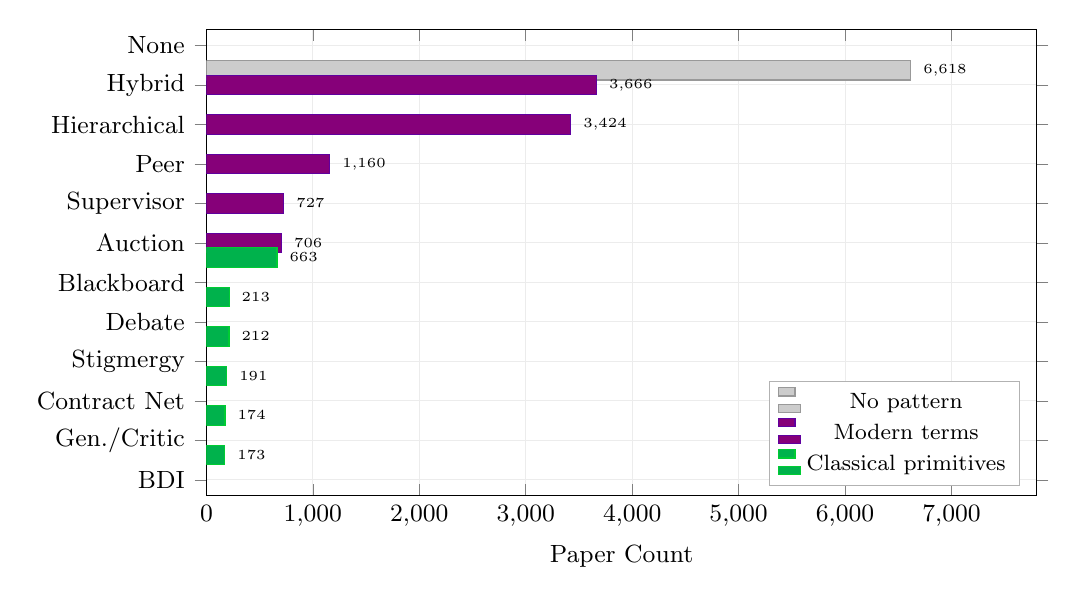
\begin{tikzpicture}
\begin{axis}[
    xbar,
    width=\columnwidth,
    height=7.5cm,
    xlabel={Paper Count},
    xlabel style={font=\small},
    xmin=0, xmax=7800,
    ytick={0,1,2,3,4,5,6,7,8,9,10,11},
    yticklabels={
        {None},
        {Hybrid},
        {Hierarchical},
        {Peer},
        {Supervisor},
        {Auction},
        {Blackboard},
        {Debate},
        {Stigmergy},
        {Contract Net},
        {Gen./Critic},
        {BDI}
    },
    yticklabel style={font=\small},
    y dir=reverse,
    bar width=7pt,
    nodes near coords,
    nodes near coords style={font=\tiny, anchor=west},
    every node near coord/.append style={xshift=1pt},
    enlarge y limits={abs=0.4},
    grid=major,
    grid style={gray!15},
    xticklabel style={font=\small},
    point meta=explicit symbolic,
    legend style={
        at={(0.98,0.02)},
        anchor=south east,
        font=\footnotesize,
        draw=black!30,
    },
]

% None (gray)
\addplot[fill=black!20, draw=black!40] coordinates {
    (6618,0) [6{,}618]
};
\addlegendentry{No pattern}

% Modern coordination terms (purple)
\addplot[fill=blue!30!purple, draw=blue!50!purple] coordinates {
    (3666,1) [3{,}666]
    (3424,2) [3{,}424]
    (1160,3) [1{,}160]
    (727,4)  [727]
    (706,5)  [706]
};
\addlegendentry{Modern terms}

% Classical primitives (green)
\addplot[fill=green!40!teal, draw=green!60!teal] coordinates {
    (663,6)  [663]
    (213,7)  [213]
    (212,8)  [212]
    (191,9)  [191]
    (174,10) [174]
    (173,11) [173]
};
\addlegendentry{Classical primitives}

\end{axis}
\end{tikzpicture}
\caption{\textbf{Coordination patterns} detected by Agent~3b across 17,955
analyzed papers. 37\% have no identifiable coordination pattern. Among
patterned papers, hybrid and hierarchical dominate. Classical primitives
(blackboard, stigmergy, contract net, BDI) appear in only 1,413
papers---the terminology has shifted even when the mechanism persists.}
\label{fig:coord-patterns}
\end{figure}


\begin{figure}[t]
\centering
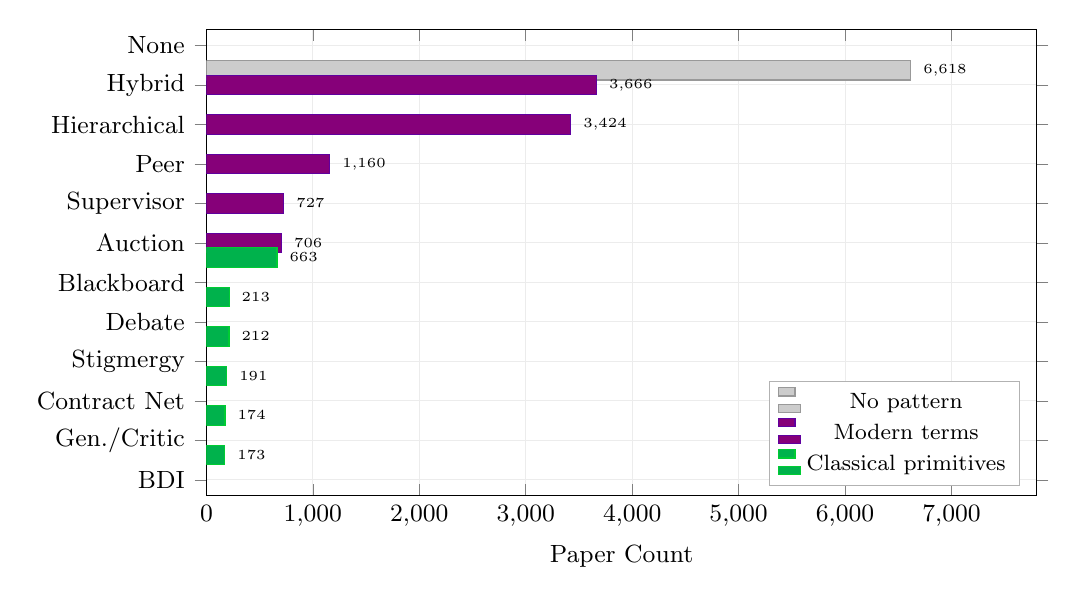
\begin{tikzpicture}
\begin{axis}[
    xbar,
    width=\columnwidth,
    height=7.5cm,
    xlabel={Paper Count},
    xlabel style={font=\small},
    xmin=0, xmax=7800,
    ytick={0,1,2,3,4,5,6,7,8,9,10,11},
    yticklabels={
        {None},
        {Hybrid},
        {Hierarchical},
        {Peer},
        {Supervisor},
        {Auction},
        {Blackboard},
        {Debate},
        {Stigmergy},
        {Contract Net},
        {Gen./Critic},
        {BDI}
    },
    yticklabel style={font=\small},
    y dir=reverse,
    bar width=7pt,
    nodes near coords,
    nodes near coords style={font=\tiny, anchor=west},
    every node near coord/.append style={xshift=1pt},
    enlarge y limits={abs=0.4},
    grid=major,
    grid style={gray!15},
    xticklabel style={font=\small},
    point meta=explicit symbolic,
    legend style={
        at={(0.98,0.02)},
        anchor=south east,
        font=\footnotesize,
        draw=black!30,
    },
]

% None (gray)
\addplot[fill=black!20, draw=black!40] coordinates {
    (6618,0) [6{,}618]
};
\addlegendentry{No pattern}

% Modern coordination terms (purple)
\addplot[fill=blue!30!purple, draw=blue!50!purple] coordinates {
    (3666,1) [3{,}666]
    (3424,2) [3{,}424]
    (1160,3) [1{,}160]
    (727,4)  [727]
    (706,5)  [706]
};
\addlegendentry{Modern terms}

% Classical primitives (green)
\addplot[fill=green!40!teal, draw=green!60!teal] coordinates {
    (663,6)  [663]
    (213,7)  [213]
    (212,8)  [212]
    (191,9)  [191]
    (174,10) [174]
    (173,11) [173]
};
\addlegendentry{Classical primitives}

\end{axis}
\end{tikzpicture}
\caption{\textbf{Coordination patterns} detected by Agent~3b across 17,955
analyzed papers. 37\% have no identifiable coordination pattern. Among
patterned papers, hybrid and hierarchical dominate. Classical primitives
(blackboard, stigmergy, contract net, BDI) appear in only 1,413
papers---the terminology has shifted even when the mechanism persists.}
\label{fig:coord-patterns}
\end{figure}


\begin{figure}[t]
\centering
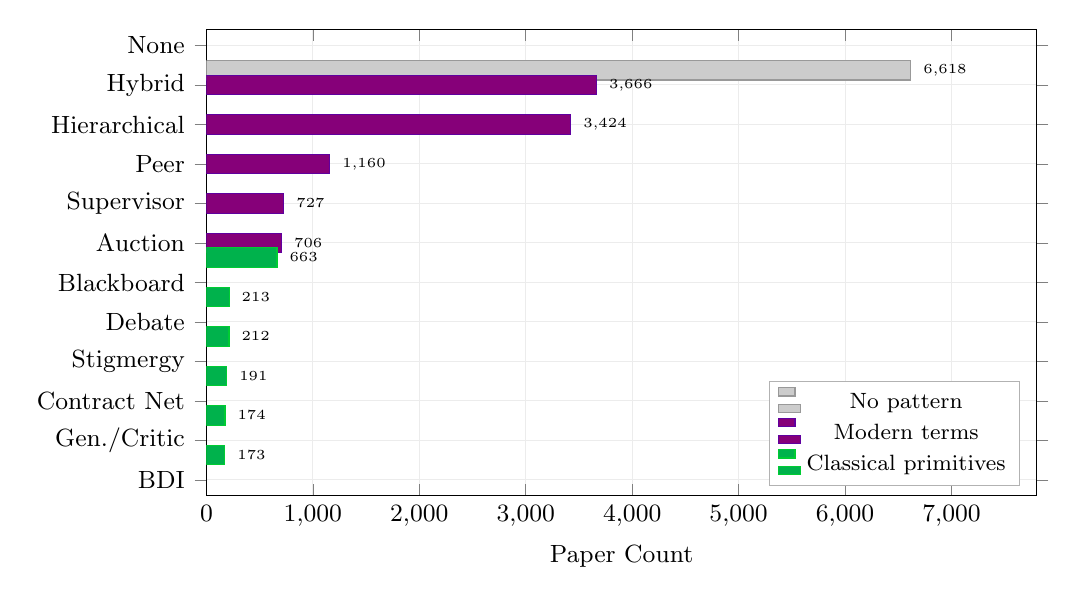
\begin{tikzpicture}
\begin{axis}[
    xbar,
    width=\columnwidth,
    height=7.5cm,
    xlabel={Paper Count},
    xlabel style={font=\small},
    xmin=0, xmax=7800,
    ytick={0,1,2,3,4,5,6,7,8,9,10,11},
    yticklabels={
        {None},
        {Hybrid},
        {Hierarchical},
        {Peer},
        {Supervisor},
        {Auction},
        {Blackboard},
        {Debate},
        {Stigmergy},
        {Contract Net},
        {Gen./Critic},
        {BDI}
    },
    yticklabel style={font=\small},
    y dir=reverse,
    bar width=7pt,
    nodes near coords,
    nodes near coords style={font=\tiny, anchor=west},
    every node near coord/.append style={xshift=1pt},
    enlarge y limits={abs=0.4},
    grid=major,
    grid style={gray!15},
    xticklabel style={font=\small},
    point meta=explicit symbolic,
    legend style={
        at={(0.98,0.02)},
        anchor=south east,
        font=\footnotesize,
        draw=black!30,
    },
]

% None (gray)
\addplot[fill=black!20, draw=black!40] coordinates {
    (6618,0) [6{,}618]
};
\addlegendentry{No pattern}

% Modern coordination terms (purple)
\addplot[fill=blue!30!purple, draw=blue!50!purple] coordinates {
    (3666,1) [3{,}666]
    (3424,2) [3{,}424]
    (1160,3) [1{,}160]
    (727,4)  [727]
    (706,5)  [706]
};
\addlegendentry{Modern terms}

% Classical primitives (green)
\addplot[fill=green!40!teal, draw=green!60!teal] coordinates {
    (663,6)  [663]
    (213,7)  [213]
    (212,8)  [212]
    (191,9)  [191]
    (174,10) [174]
    (173,11) [173]
};
\addlegendentry{Classical primitives}

\end{axis}
\end{tikzpicture}
\caption{\textbf{Coordination patterns} detected by Agent~3b across 17,955
analyzed papers. 37\% have no identifiable coordination pattern. Among
patterned papers, hybrid and hierarchical dominate. Classical primitives
(blackboard, stigmergy, contract net, BDI) appear in only 1,413
papers---the terminology has shifted even when the mechanism persists.}
\label{fig:coord-patterns}
\end{figure}
